\lecdate{07.11.2017}
Aufbau:
\begin{center}
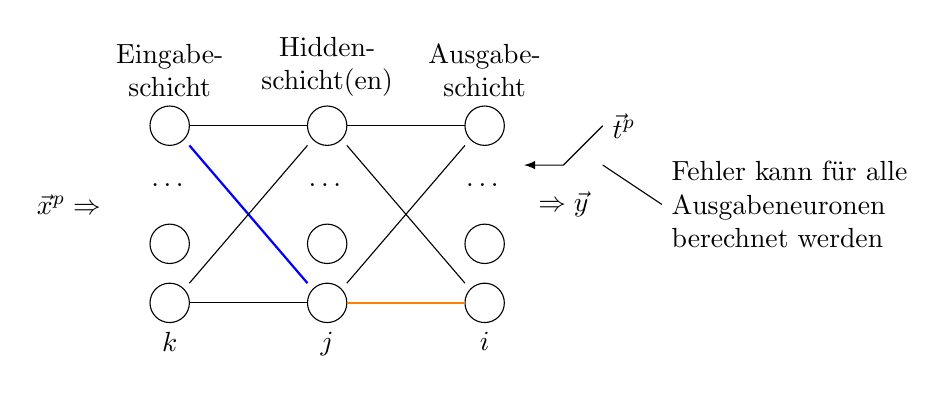
\begin{tikzpicture}[scale=.5]
\draw  (0,4) circle (0.5);
\draw  (0,1) circle (0.5);
\draw  (0,-0.5) circle (0.5);
\draw  (4,4) circle (0.5);
\draw  (4,1) circle (0.5);
\draw  (4,-0.5) circle (0.5);
\draw  (8,4) circle (0.5);
\draw  (8,1) circle (0.5);
\draw  (8,-0.5) circle (0.5);
\node at (0,4.5) [above, align=center] {Eingabe-\\schicht};
\node [above, align=center] at (4,4.5) {Hidden-\\schicht(en)};
\node [above, align=center] at (8,4.5) {Ausgabe-\\schicht};
\draw (0.5,4) -- (3.5,4);
\draw (4.5,4) -- (7.5,4);
\draw (0.5,-0.5) -- (3.5,-0.5);
\draw [thick, orange](4.5,-0.5) -- (7.5,-0.5);
\draw [thick, blue](0.5,3.5) -- (3.5,0);
\draw (0.5,0) -- (3.5,3.5);
\draw (4.5,3.5) -- (7.5,0);
\draw (4.5,0) -- (7.5,3.5);
\node at (4,2.5) {…};
\node at (0,2.5) {…};
\node at (8,2.5) {…};
\node at (0,-1) [below] {$k$};
\node at (4,-1) [below] {$j$};
\node at (8,-1) [below] {$i$};
\node at (-1.5,2) [left] {$\vec{x}^p \Rightarrow$};
\node at (11,4) [right] {$\vec{t}^p$};
\node at (10,2) {$\Rightarrow\vec{y}$};
\draw [-latex] (11,4) -- (10,3) -- (9,3);
\draw (11,3) -- (12.5,2) node[right, align=left]{Fehler kann für alle \\Ausgabeneuronen \\berechnet werden};
\end{tikzpicture}
\end{center}

\begin{itemize}
\item Feed-forward-network
\item vollvernetzt zwischen benachbarten Ebenen
\end{itemize}
Fehlerfunktion lautet:
$$\boxed{E^p = \frac{1}{2} \sum_{i=1}^{I}(t_i^p-y_i^p)^2}$$
(Quadratischer Ausgabefehler)\bigskip\\
Für alle Neuronen, ausgenommen die Eingabeneuronen, gilt:\\
$z_s = \sum w_{rs} \cdot y_s \To$ Skalarprodukt\\
$y_s = \frac{1}{1+e^{-z_s}}$\begin{center}
\begin{tikzpicture}
\begin{axis}[hide axis, axis equal, clip=false, scale=.7]
\addplot[domain=-2:2] {1/(1+e^(-4*x))}; 
\draw [-latex](-2.5,0) -- (2.5,0) node[below left]{$z_s$};
\draw [-latex](0,-0.1) -- (0,1.5) node[above right]{$y_s$}; 
\draw (0.1,1) -- (-0.1,1) node[left]{$1$};
\end{axis}
\end{tikzpicture}
\end{center}\bigskip
Für ausgezeichnetes Gewicht \torange{$w_{ji}$} würde mit Hilfe der Delta-Lernregel gelten:
$$\Delta w_{ji}=\eta \cdot y_j \cdot (t_i-y_i)$$
Wie adaptiert man das Gewicht \tblue{$w_{kj}$}?!

Idee: Die Delta-Lernregel mit Hilfe eines Gradientenverfahrens verallgemeinern, so dass sich ausgehend vom Fehler am NW-Ausgang \emph{alle} Parameter adaptieren lassen.\\
$\To$ wir notieren die Fehlerfunktion als Funktion, die vom zu adaptierenden Parameter abhängt (als Argument der Funktion). Zum Beispiel:
$$E^p(\vec{x}^p, \vec{W})=\torange{f(w_{ji})}$$
$$E^p(\vec{x}^p, \vec{W})=\tblue{f(w_{kj})}$$
$$E=\frac{1}{2}\sum(t_i-y_i)^2 =  \ldots =f(w_{ji})$$

Für alle Trainingsmuster/-beispiele soll der Fehler (am Ausgang) minimal sein. Dafür muss eben der Wert für die einzelnen Parameter der Übergänge gesucht werden, für die die Ausgabe einen minimalen Fehler hat.

Zum Bestimmen von $f(w_{ji})$ muss folgendes beachtet werden:

$\Delta w \approx -\frac{\partial E}{\partial w}$ (zum Suchen $w_{opt}$ in Richtung des Minimums bewegen)\\
$\to$ $\Delta w_{ji}\approx -\frac{\partial E}{\partial w-{ji}}$ \qquad $\Delta w_{kj}\approx - \frac{\partial E}{\partial w_{kj}}$\\
Wie hängt die Fehlerfunktion $E$ von Parameter $w_{ji}$ ab?\\
$\to$ $E_i=f(y_i)$ \quad $y_i=f(z_i)$ \quad $z_i=f(w_{ji})$\\
$\To E_i(y_i(z_i(w_{ji})))$\\
$\frac{\partial E_i}{\partial w_{ji}} = \frac{\partial E_i}{\partial y_i} \cdot \frac{\partial y_i}{\partial z_i} \cdot \frac{\partial z_i}{\partial w_{ji}}$ (Kettenregel)
\begin{itemize}
\item $\frac{\partial E_i}{\partial y_i}=\left[\frac{1}{2}(t_i-y_i)^2\right]_{y_i}=-(t_i -y_i)$
\item $\frac{\partial y_i}{\partial z_i}=\left[ \frac{1}{1+e^{-z_i}}\right]_{z_i}=\left[ (1+e^{-z_i})^{-1}\right]_{z_i}=-e^{-z_i}\cdot -(1+e^{-z_i})^{-2}\\
=\frac{e^{-z_i}}{(1+e^{-z_i})^2}=\frac{1}{1+e^{-z_i}}\cdot\frac{e^{-z_i}\torange{+1-1}}{1+e^{z_i}}=\frac{1}{1+e^{-z_i}}\cdot\left(\frac{1+e^{-z_i}}{1+e^{z_i}}-\frac{1}{1+e^{-z_i}}\right)=y_i(1-y_i)$
\item $\frac{\partial z_i}{\partial w_{ji}}=\left[ y_1^H \cdot w_{1i} + y_2^H \cdot w_{2i} + \ldots + y_j^H \cdot w_{ji} + \ldots \right]_{w_{ji}}=y_j^H$
\end{itemize}
Damit gilt:\\
$\frac{\partial E_i}{\partial w_{ji}}=-(t_i-y_i)\cdot y_i (1-y_i) \cdot y_i$\\
$\boxed{\Delta w_{ji}=\eta \left( - \frac{\partial E_i}{\partial w_{ji}} \right)}$\\
$\boxed{\Delta w_{ji} = \eta \cdot (t_i-y_i) \cdot y_i (1-y_i) \cdot y_j}$\\
Für $\Delta w_{kj}$ ergibt sich jetzt $E(y_i(z_i(y_j(z_j(w_{kj})))))$:\\
$\frac{\partial E}{\partial w_{jk}} = \frac{\partial E}{\partial y_i} \cdot \frac{\partial y_i}{\partial z_i} \cdot \frac{\partial z_i}{\partial y_j}\cdot \frac{\partial y_j}{\partial z_j}\cdot \frac{\partial z_j}{\partial w_{kj}}$\\
$\frac{\partial E}{\partial w_{jk}}= (-1) \sum_i (t_i-y_i) \cdot y_i(1-y_i) \cdot w_{ji} \cdot y_j(1-y_j) \cdot y_k$\\
Dabei sei $\boxed{ \delta_i =(t_i-y_i) \cdot y_i(1-y_i)}$ der Fehler am Knoten $i$.\\
Somit ist $\frac{\partial E}{\partial w_{jk}}=(-1) \sum_i \delta_i \cdot w_{ji} \cdot y_j(1-y_j) \cdot y_k$\\
Dabei sei $\sum_i \delta_i \cdot w_{ji} \cdot y_j(1-y_j) = \delta_j$ der Fehler am Knoten $j$.\\
Somit ist $\Delta w_{kj}=\eta \cdot y_j(1-y_j) \cdot y_k \sum_i \delta _i \cdot w_{ji} = \eta \cdot \delta_j \cdot y_k$\\
$\boxed{\Delta w_{ji}=\eta \cdot \delta_i \cdot y_j}$
$\boxed{\Delta w_{kj}=\eta \cdot \delta_j \cdot y_k}$ usw.






\section{Beispiel}
%%% Handout
Wichtig: An Neuron wird der $z$-Wert zusammengerechnet. Für die folgenden Neuronen ist dann der $y$-Wert relevant, der sich aus dem $z$-Wert ergibt.
\begin{align*}
z_5 &= 0,6\cdot 0 &&+ 0,3 \cdot 1 &&+ 0,1 \cdot 0 &&+ (-0,3) \cdot 1 &&+ 0 &&= 0\\
z_6 &= 0,1\cdot 0 &&+ 0,1 \cdot 1 &&+ 0,1 \cdot 0 &&+ 0,1 \cdot 1 &&-0,2 &&= 0\\
z_7 &= 0,4\cdot 0 &&+ (-0,1) \cdot 1 &&+ 0,1 \cdot 0 &&+ (-0,2) \cdot 1 &&+ 0,3 &&= 0
\end{align*}

\lecdate{14.11.2017}
Wichtig: Eingangsvariable $\vec{x}^p$ und Vorgabe $\vec{t}^p$.\\
Ergebnis im Vergleich zur Vorgabe:\\
$\vec{y}^p=\mtr{y_8\\y_9}=\mtr{0,5\\0,5} \Leftrightarrow \vec{t}^p = \mtr{t_8\\t_9}=\mtr{0\\1}$
\begin{center}
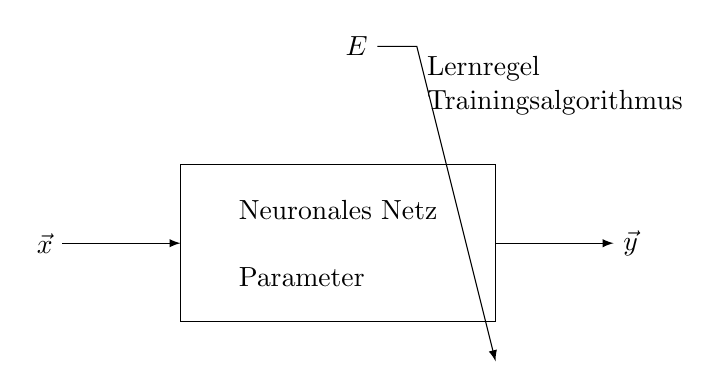
\begin{tikzpicture}
\draw  (-4,3) rectangle node[align=left]{Neuronales Netz\\\\ Parameter} (0,1);
\draw [-latex] (-5.5,2) node[left]{$\vec{x}$} -- (-4,2);
\draw [-latex] (0,2) -- (1.5,2) node[right]{$\vec{y}$};
\draw [-latex] (-1.5,4.5) node[left]{$E$} -- (-1,4.5) node[below right = .2, align=left]{Lernregel\\Trainingsalgorithmus} -- (0,0.5);
\end{tikzpicture}
\end{center}
$$\Delta w(t) = \eta \cdot \left( -\frac{\partial E}{\partial w}\right)$$
$$w(t+1) = w(t) + \Delta w(t)$$
Beispielweg von einem Eingang zum Ausgang:\\
$\Delta w_{58}=\eta \cdot \delta_8 \cdot y_5$ mit $\delta_8 = \underbrace{(t_8-y_8)}_{F'(y_8)\cdot (-1)} \cdot \underbrace{y_8 \cdot (1-y_8)}_{F'(z_8)}$\\
$\Delta w_{15}=\eta\cdot \delta_5 \cdot y_1$ mit $\delta_5 = (w_{58}\cdot \delta_8 + w_{59} \cdot \delta_9) \cdot y_5 \cdot (1-y_5)$\\
Damit lässt sich berechnen:
\subsection{Erster Trainingsschritt}
Gesucht: $\Delta \vec{w}_8$, $\Delta\vec{w}_9$, $\Delta\vec{w}_5$, $\Delta\vec{w}_6$, $\Delta\vec{w}_7$ (Training)
\begin{itemize}
\item $\Delta \vec{w}_8 = (\Delta w_{B8},\; \Delta w_{58},\; \Delta w_{68},\; \Delta w_{78})^T$
\begin{itemize}
\item $\Delta w_{B8} = 0,1 \cdot (0-0,5) \cdot 0,5 \cdot (1-0,5) \cdot 1 = -0,0125$
\item $\Delta w_{58} = 0,1 \cdot \underbrace{(0-0,5)\cdot 0,5\cdot (1-0,5)}_{\delta_8=-0,125} \cdot 0,5 = -0,00625$
\item $\Delta w_{68} = \Delta w_{58}$
\item $\Delta w_{78} = \Delta w_{58}$
\end{itemize}
\item $\Delta \vec{w}_9 = (\Delta w_{B9},\; \Delta w_{59},\; \Delta w_{69},\; \Delta w_{79})^T$
\begin{itemize}
\item $\Delta w_{B9} = 0,0125$
\item $\Delta w_{59} = 0,1 \cdot \underbrace{(1-0,5) \cdot 0,5 \cdot (1-0,5)}_{\delta_9=0,125} \cdot 0,5 = 0,00625$
\item $\Delta w_{69} = \Delta w_{59}$
\item $\Delta w_{79} = \Delta w_{59}$
\end{itemize}
\item $\Delta \vec{w}_5 = (w_{B5},\; w_{15},\; w_{25},\; w_{35},\; w_{45})^T$
\begin{itemize}
\item $\Delta w_{B5} = 0,1 \cdot \underbrace{[(-0,6) \cdot (-0,125) + (-0,6) \cdot 0,125]}_{=0}\cdot 0,5 \cdot (1-0,5) \cdot 0 = 0$
\item $\Delta w_{15} = 0$
\item $\Delta w_{25} = 0$
\item $\Delta w_{35} = 0$
\item $\Delta w_{45} = 0$
\end{itemize}
\item $\Delta \vec{w}_6 = (w_{B6},\; w_{16},\; w_{26},\; w_{36},\; w_{46})^T$
\begin{itemize}
\item $\Delta w_{B6} = 0,1 \cdot [0,2 \cdot (-0,125) + (-0,4) \cdot 0,125]\cdot 0,5 \cdot (1-0,5) \cdot 1 = -0,001875$
\item $\Delta w_{16} = 0$
\item $\Delta w_{26} = \Delta w_{B6}$
\item $\Delta w_{36} = 0$
\item $\Delta w_{46} = \Delta w_{B6}$
\end{itemize}
\item $\Delta \vec{w}_7 = (w_{B7},\; w_{17},\; w_{27},\; w_{37},\; w_{47})^T$
\begin{itemize}
\item $\Delta w_{B7} = 0,1 \cdot [(-0,6) \cdot (-0,125) + (-0,4) \cdot 0,125]\cdot 0,5 \cdot (1-0,5) \cdot 1 = -0,000625$
\item $\Delta w_{17} = 0$
\item $\Delta w_{27} = \Delta w_{B7}$
\item $\Delta w_{37} = 0$
\item $\Delta w_{47} = \Delta w_{B7}$
\end{itemize}
\end{itemize}
Optionen beim Korrigieren: Entweder Änderungen direkt drauf rechnen (direct learning), oder als zusätzlichen „Delta-Bias“ in einer Variable speichern und dann drauf rechnen (batch learning).

Warum initialisieren wir die Parameter mit \emph{zufälligen} Werten?
% Folien: Übung, Folien 5+6
\begin{itemize}
\item Damit die Änderungen möglichst nicht klein werden.
\end{itemize}
Was passiert, wenn alle Parameter mit Null initialisiert werden?
\begin{itemize}
\item $z_5=z_6=z_7=0$
\item $y_5=y_6=y_7=0.5$
\item $z_8=z_9=0$
\item $y_8=y_9=0.5$
\end{itemize}
$\to$ die $y$-Werte bleiben gleich.\\
Beim Training:\\
1.Schritt:
\begin{itemize}
\item $\Delta \vec{w}_8$ und $\Delta \vec{w}_9$ bleiben wie bei der zufälligen Verteilung.
\item $\Delta \vec{w}_5=\Delta \vec{w}_6=\vec{w}_7$ ist dann $\vec{0}$.
\end{itemize}
Damit:
\begin{itemize}
\item $\vec{w}_8(t+1)=\vec{w}_8(t)+\Delta w_8(t) = (-0,0125, -0,00625,\ldots)^T$
\item $\vec{w}_9(t+1)=\vec{w}_9(t)+\Delta w_9(t) = (0,0125, 0,00625,\ldots)^T$
\item $\vec{w}_4(t+1) = \vec{w}_4(t)$, gleiches für $\vec{w}_5$ und $\vec{w}_6$
\end{itemize}
Und somit:
\begin{itemize}
\item $z_5=z_6=z_7= 0$
\item $y_5=y_6=y_7 = 0.5$
\item $z_8=-0.0125\cdot 1 + 3 \cdot ((-0.00625)\cdot  0.5)=-0.021875$
\item $z_9=0.0125\cdot 1 + 3 \cdot (0.00625\cdot  0.5)=0.021875$
\item $y_8=0.5055$
\item $y_9=0.4945$
\end{itemize}
2. Schritt:
\begin{itemize}
\item $\Delta\vec{w}_8=(-0.0124,-0.0062,-0.0062,\ldots)^T$
\item $\Delta\vec{w}_9=(0.0124, 0.0062,0.0062,\ldots)^T$
\item $\Delta \vec{w}_5=\Delta \vec{w}_6 = \Delta\vec{w}_7 = (0.00004, 0, 0.00004, 0, 0.00004)^T$
\end{itemize}
Damit:
\begin{itemize}
\item $\vec{w}_5(t+2)=\vec{w}_6(t+2)=\vec{w}_7(t+2)=(0.00004, 0, 0.00004, 0, 0.00004)$
\end{itemize}
$\to$ alle Hidden-Knoten sind gleich $\to$ man könnte die Hidden-Knoten auch auf einen reduzieren. Damit kann aber bspw. nur eine Gerade abgebildet werden (Vergleich XOR -- braucht 2 Geraden) (vgl. Symmetriebruch).\\
$\To$ man braucht unterschiedliche/zufällige Initialwerte, damit \emph{unterschiedliche} Geraden angelernt werden können!

\section{Multi Layered Perceptron}
\slides{NI_WS2017_Kap3_MLP}{1}

\section{Grundprinzip Training}
\slides{NI_WS2017_Kap3_MLP}{2}

\section{Error-Backtracking-Algorithmus}
\slides{NI_WS2017_Kap3_MLP}{3}
\subsection{Gradientanstieg}
\slides{NI_WS2017_Kap3_MLP}{4}
\subsection{Rückpropagierung des Fehlers am Netzwerk-Ausgang}
\slides{NI_WS2017_Kap3_MLP}{5}
\slides{NI_WS2017_Kap3_MLP}{6}
\subsection{Adaptionsvorschriften}
\slides{NI_WS2017_Kap3_MLP}{7}
\subsection{Fazit}
\slides{NI_WS2017_Kap3_MLP}{8}

